\chapter{Installation}
\label{chap:installation}

\section{Install Our Extension for Enterprise Architect}
Enterprise Architect (EA) is a modelling tool that supports UML\footnote{Unified Modelling Language} and a host of other modelling languages.
EA is not only affordable but is also quite flexible and can be extended via \emph{extensions} to support new modelling languages.
\begin{enumerate}
\item[$\blacktriangleright$] Download EA for Windows from \url{http://www.sparxsystems.com/} to get a free 30 day trial and follow installation instructions (Fig.~\ref{fig_enterpriseArchitextHomepage}).

\begin{figure}[htbp]
	\centering
  	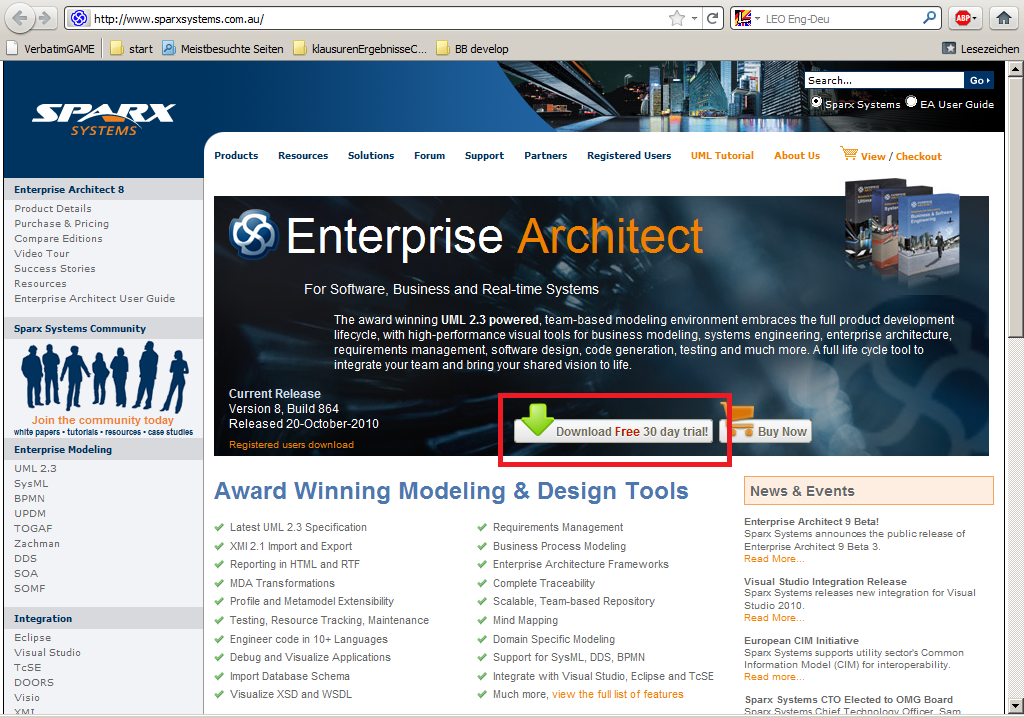
\includegraphics[width=0.77\textwidth]{pics/installationAndSetup/ea_download.png}
	\caption{Download Enterprise Architect}
	\label{fig_enterpriseArchitextHomepage}
\end{figure} 

\item[$\blacktriangleright$] Install our EA-Extension (Fig.~\ref{fig_eaPluginWizard}) to add support for our modelling languages.
Download \url{http://www.moflon.org/fileadmin/download/moflon-ide/eclipse-plugin/ea-ecore-addin/ea-ecore-addin.zip}, unpack, and run \texttt{setup.exe}.

\begin{figure}[htbp]
	\centering
  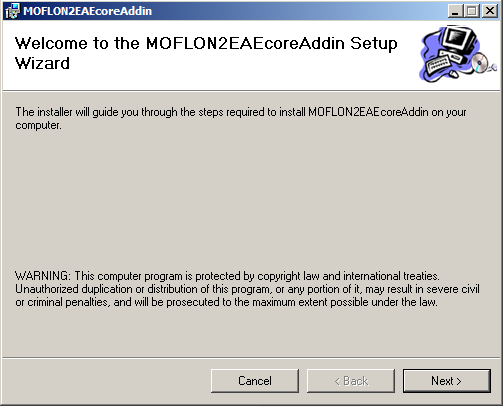
\includegraphics[width=0.5\textwidth]{pics/installationAndSetup/eaplugin_install.png}
	\caption{Install our extension for EA}
	\label{fig_eaPluginWizard}
\end{figure}
\end{enumerate}
 
\section{Install Our Plugin for Eclipse}
\begin{enumerate}
\item[$\blacktriangleright$] Download and install Eclipse for Modelling ``Eclipse Modeling Tools (includes incubating components)''\footnote{Please note that you \emph{have to} install \emph{Eclipse Modeling Tools} or nothing will work.  Do not choose a different Eclipse package!  Although different versions and constellations might work, eMoflon is currently tested for Eclipse Juno and Java 1.7.} from \url{http://www.eclipse.org/downloads/packages/} (Fig.~\ref{fig_downloadModelingPackage}).

\begin{figure}[htbp]
	\centering
  	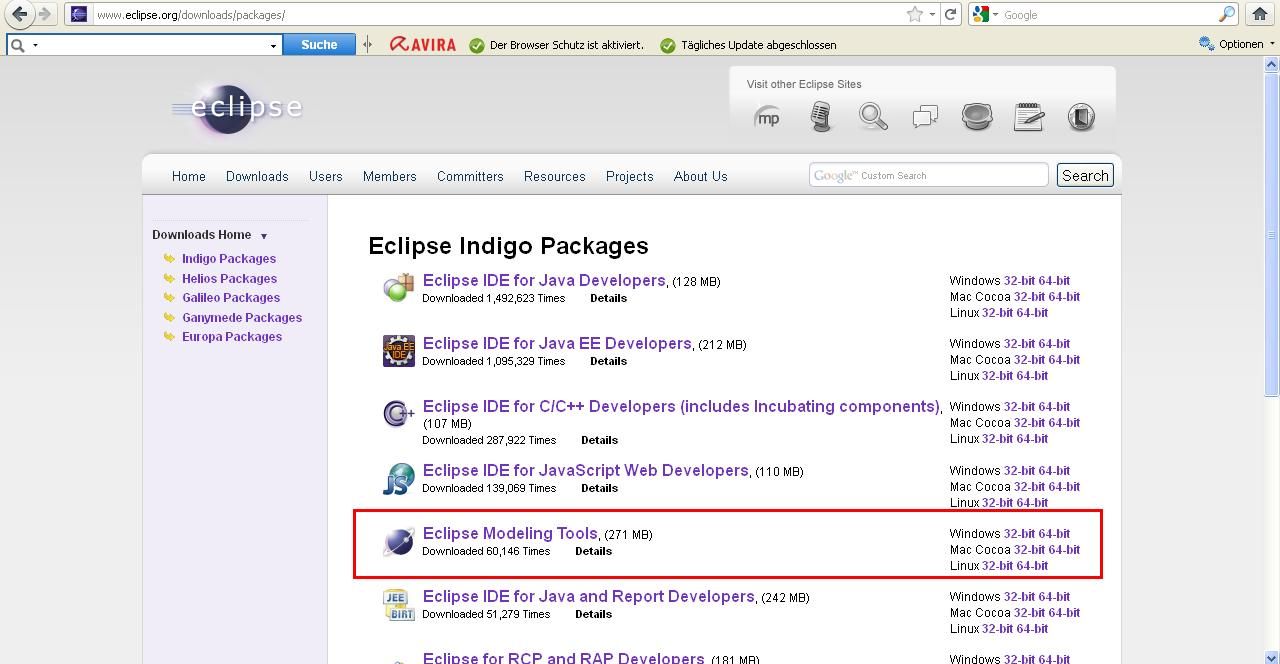
\includegraphics[width=0.85\textwidth]{pics/installationAndSetup/eclipse_modelingpackage.png}
	\caption{Download Eclipse Modeling Tools.}
	\label{fig_downloadModelingPackage}
\end{figure}

\item[$\blacktriangleright$] Install our Eclipse Plugin from the following update site\footnote{For a detailed tutorial on how to install Eclipse and Eclipse Plugins please refer to \url{http://www.vogella.de/articles/Eclipse/article.html}} 
\footnote{Please note: Calculating requirements and dependencies when installing the plugin might take quite a while depending on your internet connection.}:
\url{http://www.moflon.org/fileadmin/download/moflon-ide/eclipse-plugin/update-site2}
\end{enumerate}

\section{Get a Simple Demo Running}

\begin{enumerate}
\item[$\blacktriangleright$] Go to ``Window/Open Perspective/Other\ldots''\footnote{A path given as ``foo/bar'' indicates how to navigate in a series of menus and submenus.} and choose Moflon (Fig.~\ref{fig_eclipse}). 
\begin{figure}[htbp]
	\centering
  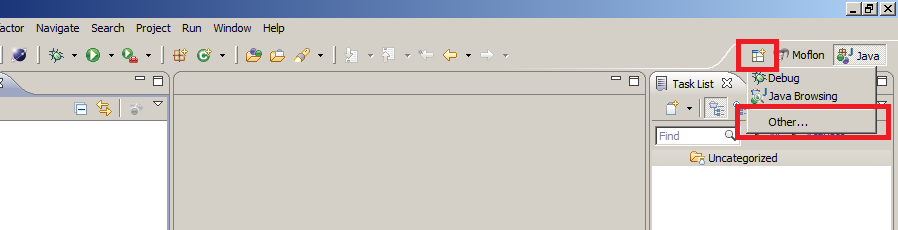
\includegraphics[width=\textwidth]{pics/installationAndSetup/eclipse_firststart.png}
	\caption{Choose the Moflon Perspective.}
	\label{fig_eclipse}
\end{figure}

\item[$\blacktriangleright$] In the toolbar a new action set should have appeared. Choose ``New Metamodel'' (Fig.~\ref{fig_eclipseNewMetamodel}).
The button with an ``L" shows you our logfile (important input for us if something goes wrong!).
\begin{figure}[htbp]
	\centering
  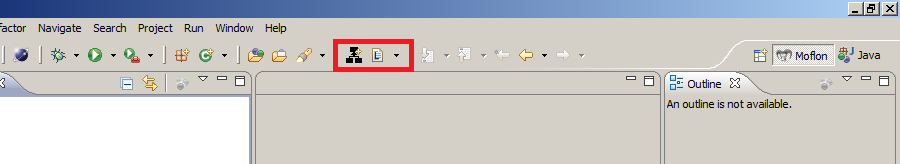
\includegraphics[width=\textwidth]{pics/installationAndSetup/eclipse_metamodelButton.png}
	\caption{Eclipse New Metamodel}
	\label{fig_eclipseNewMetamodel}
\end{figure}

\item[$\blacktriangleright$] Enter ``Demo'' as the name of the new metamodel project and confirm. 
An empty EA project file ``Demo.eap'' will be created in a new project with a certain project structure according to our conventions\footnote{At the moment, the project contains only the EA project file.}.
Please do not rename, move or delete anything.

\item[$\blacktriangleright$] Choose working sets as your top level element in the package explorer (Fig.~\ref{fig_eclipseWorkingsets}).
We work a lot with working sets and use them to structure the workspace in Eclipse.
\begin{figure}[htbp]
	\centering
  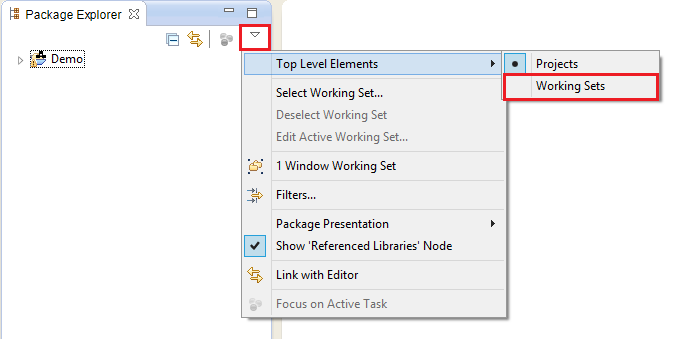
\includegraphics[width=0.9\textwidth]{pics/installationAndSetup/eclipse_workingsets.png}
	\caption{Choose Working Sets as Top Level Elements.}
	\label{fig_eclipseWorkingsets}
\end{figure} 

\item[$\blacktriangleright$] Open the newly created project and replace the ``Demo.eap'' file with the Demo.eap that you will find in the \texttt{eMoflonTutorial.zip} file provided together with this tutorial. 

\item[$\blacktriangleright$] Double click ``Demo.eap'' to start EA.
Please choose ``Ultimate" when starting EA for the first time.

\item[$\blacktriangleright$] In EA, choose ``Extensions/MOFLON::Ecore Addin/Export\- all\- to\- Workspace'' (Fig.~\ref{fig_ea}).
You can of course browse the project structure, but please do not rename, move or delete anything yet.
\begin{figure}[htbp]
	\centering
  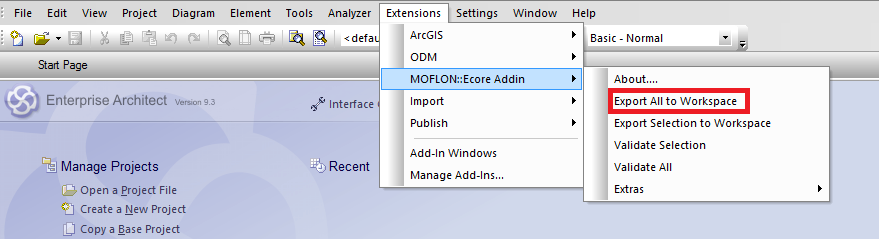
\includegraphics[width=0.9\textwidth]{pics/installationAndSetup/ea_firststart}
	\caption{Export from EA using our extension} 
	\label{fig_ea} 
\end{figure}

\item[$\blacktriangleright$] Switch back to Eclipse, choose your Metamodel project and press F5 to refresh.
The export from EA places all required files in a hidden folder in the project, and refreshing triggers a build process that invokes our code generators automatically.
You should be able to monitor the progress in the lower right corner (Fig.~\ref{fig_eclipsebuilding}).  
Pressing the symbol opens a monitor view that gives more details of the build process. 
You don't need to worry about any of these details, just remember to refresh your Eclipse workspace after an export.
\begin{figure}[htbp]
	\centering
  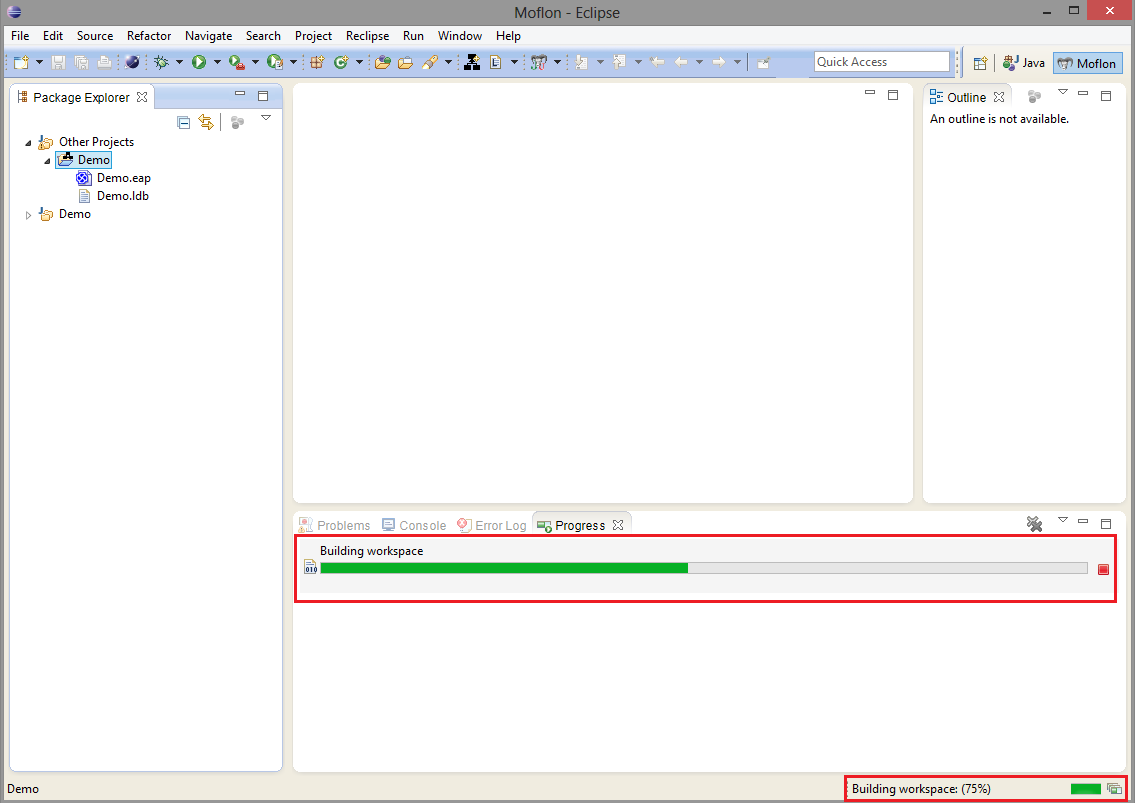
\includegraphics[width=0.55\textwidth]{pics/installationAndSetup/eclipse_building.png}
	\caption{Automatically building the workspace after a refresh.}
	\label{fig_eclipsebuilding}
\end{figure}
\end{enumerate}

\section{Validate Your Installation with JUnit}
\label{sec:junit}

\begin{enumerate}
\item[$\blacktriangleright$] Go to ``File/Import/General/Existing Projects into Workspace'' (Fig.~\ref{fig_eclipseTestsuiteImport}) and choose the Testsuite project that is also in the \texttt{eMoflonTutorial.zip} provided with this tutorial. 
\begin{figure}[htbp]
	\centering
  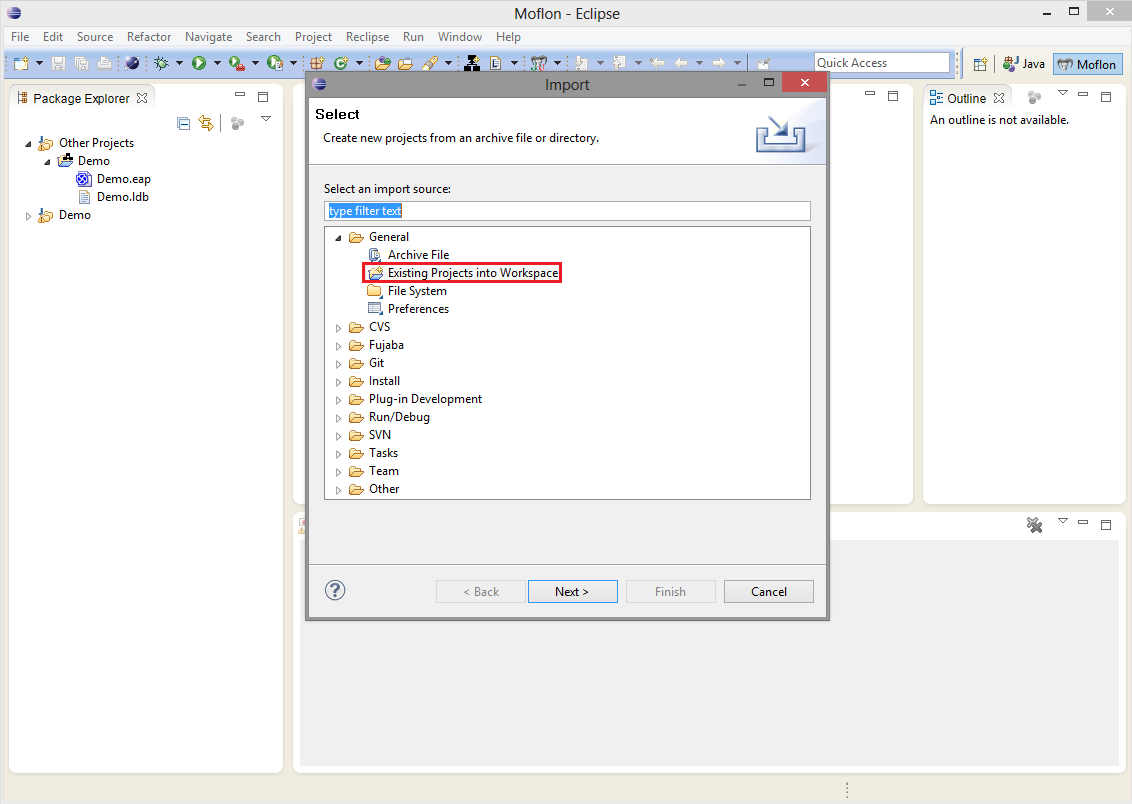
\includegraphics[width=0.55\textwidth]{pics/installationAndSetup/eclipse_testsuitimport.png}
	\caption{Import our Testsuite as an existing project.}
	\label{fig_eclipseTestsuiteImport}
\end{figure} 

\item[] At this point, your workspace should resemble Fig.~\ref{fig_eclipsepackageexplorer}.
\begin{figure}[htbp]
	\centering
  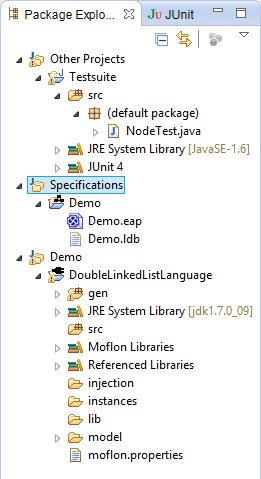
\includegraphics[width=0.4\textwidth]{pics/installationAndSetup/eclipse_packageexplorer.png}
	\caption{Workspace in Eclipse.}
	\label{fig_eclipsepackageexplorer}
\end{figure}

\item[$\blacktriangleright$] Right-click on the Testsuite project and select ``Run as/JUnit Test''.
If anything goes wrong, try refreshing your whole workspace by choosing projects and pressing \texttt{F5} or right-clicking and selecting ``Refresh''.

\begin{figure}[htbp]
	\centering
  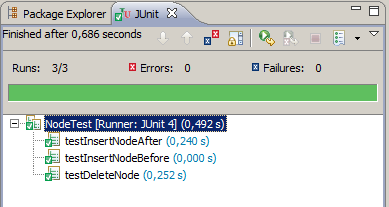
\includegraphics[width=0.5\textwidth]{pics/installationAndSetup/eclipse_testsuiterun.png}
	\caption{All's well that ends well\ldots}
	\label{fig_eclipsetestsuiterun}
\end{figure}
\end{enumerate}

Congratulations!  If you see a green bar  (Fig.~\ref{fig_eclipsetestsuiterun}), then everything has been set-up correctly and you are now ready to start metamodelling!


\section{Project Structure and Setup}
Now that everything is installed and setup properly, let's take a closer look at the different workspaces and our workflow.
Before we continue, please make a few slight adjustments to EA so you can easily compare your current workspace to our screenshots:
\begin{itemize} 

\item[$\blacktriangleright$] Select ``Tools/Options/Standard Colors'' in EA, and set your colours to reflect Fig.~\ref{fig_standardColoursEA}.
This is advisable but you're of course free to choose your own colour schema.
\begin{figure}[htbp]
  \centering
  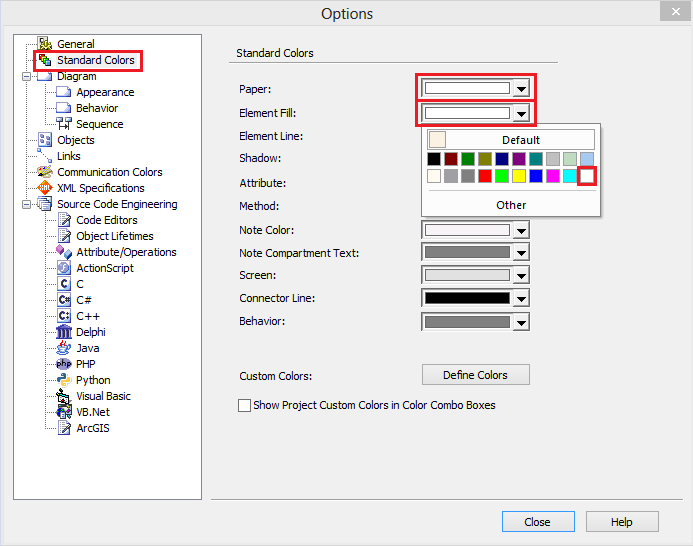
\includegraphics[width=0.8\textwidth]{pics/installationAndSetup/standardColours}
  \caption{Our choice of standard colours for diagrams in EA.}
  \label{fig_standardColoursEA}
\end{figure}

\item[$\blacktriangleright$] In the same dialogue, select ``Diagram/Appearance'' and reflect the settings in Fig.~\ref{fig_standardAppearanceEA}.
\begin{figure}[htbp]
  \centering
  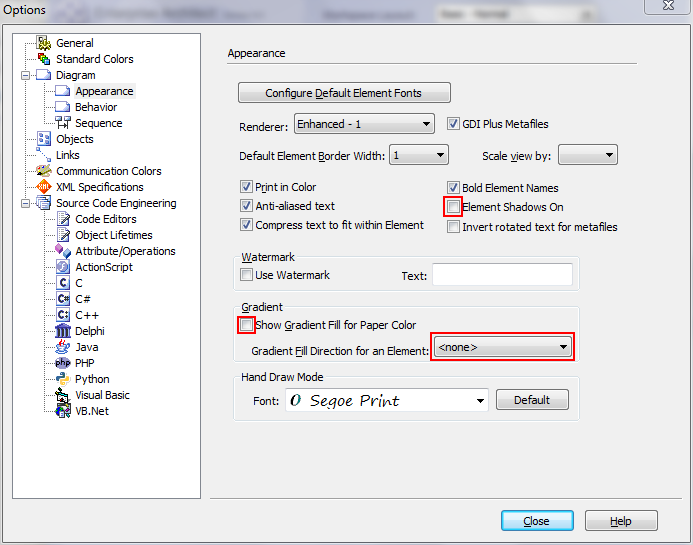
\includegraphics[width=0.8\textwidth]{pics/installationAndSetup/standardAppearance}
  \caption{Our choice of the standard appearance for model elements.}
  \label{fig_standardAppearanceEA}
\end{figure}
Again this is just a suggestion and not mandatory.

\item[$\blacktriangleright$] Last but not least, and still in the same dialogue, select ``Source Code Engineering'' and be sure to choose ``Ecore'' as the default language for code generation (Fig.~\ref{fig_standardSCEEA}). 
This setting is very important.
\begin{figure}
  \centering
  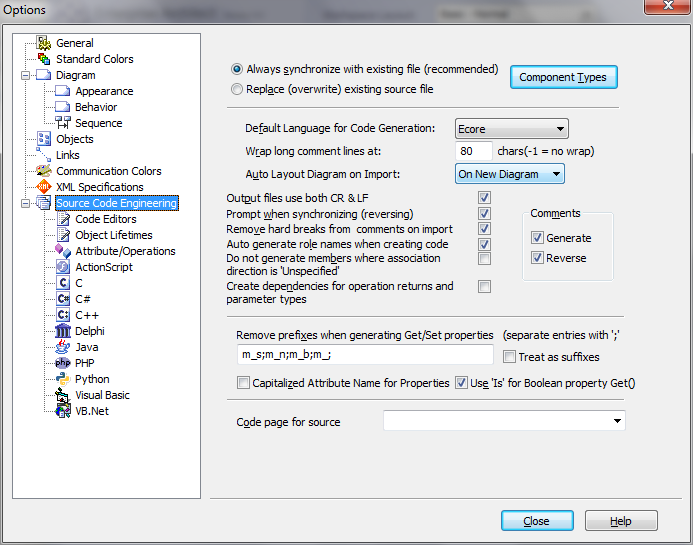
\includegraphics[width=0.8\textwidth]{pics/installationAndSetup/standardCodeEngineering}
  \caption{Make sure you set the standard language to Ecore.}
  \label{fig_standardSCEEA}
\end{figure}
\end{itemize}

In your EA ``workspace'', actually referred to as an \emph{EA project}\footnote{Words are set in italics when they represent concepts that are introduced or defined  in the corresponding paragraph for the first time.}, take a careful  look at the project structure:  The root node \texttt{Demo}\footnote{Words set  in a \texttt{mono-space font} refer to things that you should find in a tool,  dialogue, figure or code.} is called a \emph{model} in EA lingo and is used as a  container to group a set of related \emph{packages}. 
In our case, \texttt{Demo}  consists of a single package \texttt{DoubleLinkedListLanguage}.
An EA project can however consist of numerous models that in turn group  numerous packages.

Now switch to your \emph{Eclipse workspace} and note the two nodes named \texttt{Spe\-ci\-fi\-ca\-tions} and \texttt{Demo}.  These nodes, used to group related \emph{Eclipse projects} in an Eclipse workspace, are called \emph{working sets}.
The working set \texttt{Spe\-ci\-fi\-ca\-tions} contains all \emph{metamodel projects} in a  workspace.
A metamodel project contains a single EAP (EA project) file and is used to communicate with EA and initiate code generation by simply pressing F5 or choosing ``refresh'' from the context menu.
In our case, \texttt{Specifications} should contain a single metamodel project \texttt{Demo} containing our EA project file  \texttt{Demo.eap}.

\begin{figure}[htbp]
	\centering
  \includegraphics[width=\textwidth]{pics/installationAndSetup/bothexplorers}
	\caption{From EA to Eclipse}
	\label{fig_fromEAtoEclipse}
\end{figure}

Figure~\ref{fig_fromEAtoEclipse} depicts how the Eclipse working set \texttt{Demo} and its contents were generated from the EA model \texttt{Demo}.
Every model in EA is mapped to a working set in Eclipse with the same name. 
From every package in the EA model, an Eclipse project is generated, also with the same name.
These projects, however, are of a different \emph{nature} than for example metamodel projects or normal Java projects, and are called \emph{repository projects}.  
A nature is Eclipse lingo for ``project type'' and is visually indicated by a corresponding nature icon on the project folder.
Our  metamodel projects sport a spanking little class diagram symbol. 
Repository projects are generated automatically  with a certain project structure according to our conventions.  
The  \texttt{model} subfolder is probably most important, and contains an  \emph{Ecore model}.  
Ecore is a metamodelling language that provides building  blocks like \emph{classes} and \emph{references} for defining the  static structure (concepts and relations between concepts) of a system.  
The  export function of our EA plugin generates a valid Ecore model from the  corresponding EA model and persists it as an XML file in the \texttt{model}  subfolder.  
In our concrete example, this is the \texttt{DoubleLinkedListLanguage.ecore} file.  
Go ahead and double-click it to open the file in a simple tree-view editor in Eclipse.  
If you are really interested in the nitty-gritty details or have a masochistic hang, right-click the file and select ``Open With/Text Editor''. 

This Ecore model is used to drive a code generator that maps the model to Java interfaces and classes.  
The generated Java code that represents the model is often referred to as a \emph{repository} and this is the reason why we refer to such projects as repository projects\footnote{Not to be mixed up with CVS or SVN repositories, although the idea of a source code ``container'' is the same here.}. 
A repository can be viewed as an \emph{adapter} that enables building and manipulating concrete instances of a specific model via a programming language such as Java.  
This is why we indicate repository projects using a cute adapter/plug symbol on the project folder.  

Figure~\ref{fig_fromEAtoEclipse} depicts how the class \texttt{Node} in the EA model is mapped to the Java interface \texttt{Node}.  
Double-click \texttt{Node.java} and take a look at the methods declared in the interface.
These correspond directly to the methods declared in the modelled \texttt{Node} class.  
Indicated by the source folders \texttt{src} and \texttt{gen}, we advocate a clean separation of hand-written (this should go in \texttt{src}) and generated code (lands automatically in \texttt{gen}).  
As we shall see later in the tutorial, hand-written code can also be integrated directly in generated classes and, if marked appropriately, merged nicely by the code generator. 
This is sometimes more elegant for small helper functions but can quickly get problematic especially in combination with source code management systems.

If you take a careful look at the code structure in \texttt{gen}, you'll find a \texttt{Foo\-Impl.java} for every \texttt{Foo.java}. 
Indeed, the subpackage \texttt{impl} contains Java classes that implement the interfaces in the parent package.  
Although this might strike you as unnecessary (why not merge interface and implementation for simple classes?), this consequent separation in interfaces and implementation allows for a clean and relatively simple mapping of Ecore to Java, even in tricky cases like multiple inheritance (allowed and very common in Ecore models).  
A further package \texttt{util} contains some auxiliary classes such as a factory for creating instances of the model.  
If this is your first time of seeing generated code, you might be shocked at the sheer amount of classes and code generated from our relatively simple EA model.  
You might be thinking: ``hey - if I did this by hand I wouldn't need half of all this stuff!''.  
Well you're right and you're wrong -- the point is that an automatic mapping to Java via a code generator scales quite well.
This means for simple, trivial examples (like our double linked list), it might be possible to come up with a leaner and simpler Java representation.  
For complex, large models with lots of mean pitfalls, however, this becomes a daunting task.  
The code generator provides you with years and years of experience of professional programmers who have thought up clever ways of handling multiple inheritance, an efficient event mechanism, reflection, consistency between bidirectionally linked objects and much more.

A point to note here is that the mapping to Java is obviously not unique. 
Indeed there exist different standards of how to map a modelling language to a general purpose programming language like Java. 
We use a mapping defined and implemented by the Eclipse Modelling Framework (EMF) which tends to favour efficiency and simplicity.

Although getting the \emph{details} of mapping the static structure of our models to Java might be extremely difficult, it seems for the most part pretty straight  forward.  
A fantastic productivity boost in any case but (yawn) not exactly exciting.

Have you noticed the methods of the \texttt{Node} class in our EA model? 
Now hold on tight -- each method can be \emph{modelled} completely in EA and the corresponding implementation in Java is generated automatically and placed in \texttt{NodeImpl}.  
Just in case you didn't get it: The behavioural or dynamic aspects of a system can be completely modelled in an abstract, platform (programming language) independent fashion using a blend of activity  diagrams and a ``graph pattern'' language called Story Driven Modelling (SDM).  
In our EA project, these ``Stories'', ``Story Models'' or simply ``SDMs'' are  placed in SDM Containers named according to the method they implement.  
E.g.  \texttt{$\ll$ SDM Container$\gg$ insertNodeAfter SDM} for the method  \texttt{insertNodeAfter(Node)} as depicted in
Fig.~\ref{fig_fromEAtoEclipse}.  
We'll spend the rest of the tutorial understanding why SDMs are so  {\huge crazily} cool!
 
To recap all we've discussed, let's consider the complete workflow as depicted in Figure~\ref{fig_Overview}. 
We started with a concise model in EA, simple and independent of any platform specific details (1).  
Our EA model consists not only of static aspects modelled as a class diagram (2), but also of dynamic
aspects modelled using SDM (3).  After exporting the model and code generation (4), we basically switch from \emph{modelling} to \emph{programming} in a specific general purpose programming language (Java).  
On this lower \emph{level of abstraction}, we can flesh out the generated repository (5) if necessary, and mix as appropriate with hand-written code and libraries.  Our abstract specification of behaviour (methods) in SDM is translated to a series of method calls that form the body of the corresponding Java method (6).

If you feel a bit lost at the moment please be patient; this first chapter has been a lot about installation and tool support and only aims at giving a very brief glimpse at the big picture of what is actually going on.    

In the following chapter, we shall go step-by-step through a hands-on example and cover the core features of Ecore (static structure) and SDM (behaviour). 
We shall also give clear and simple definitions for the most important metamodelling and graph transformation concepts, always referring to the concrete example and providing lots of references for further reading.

\begin{figure}[htbp]
	\centering
  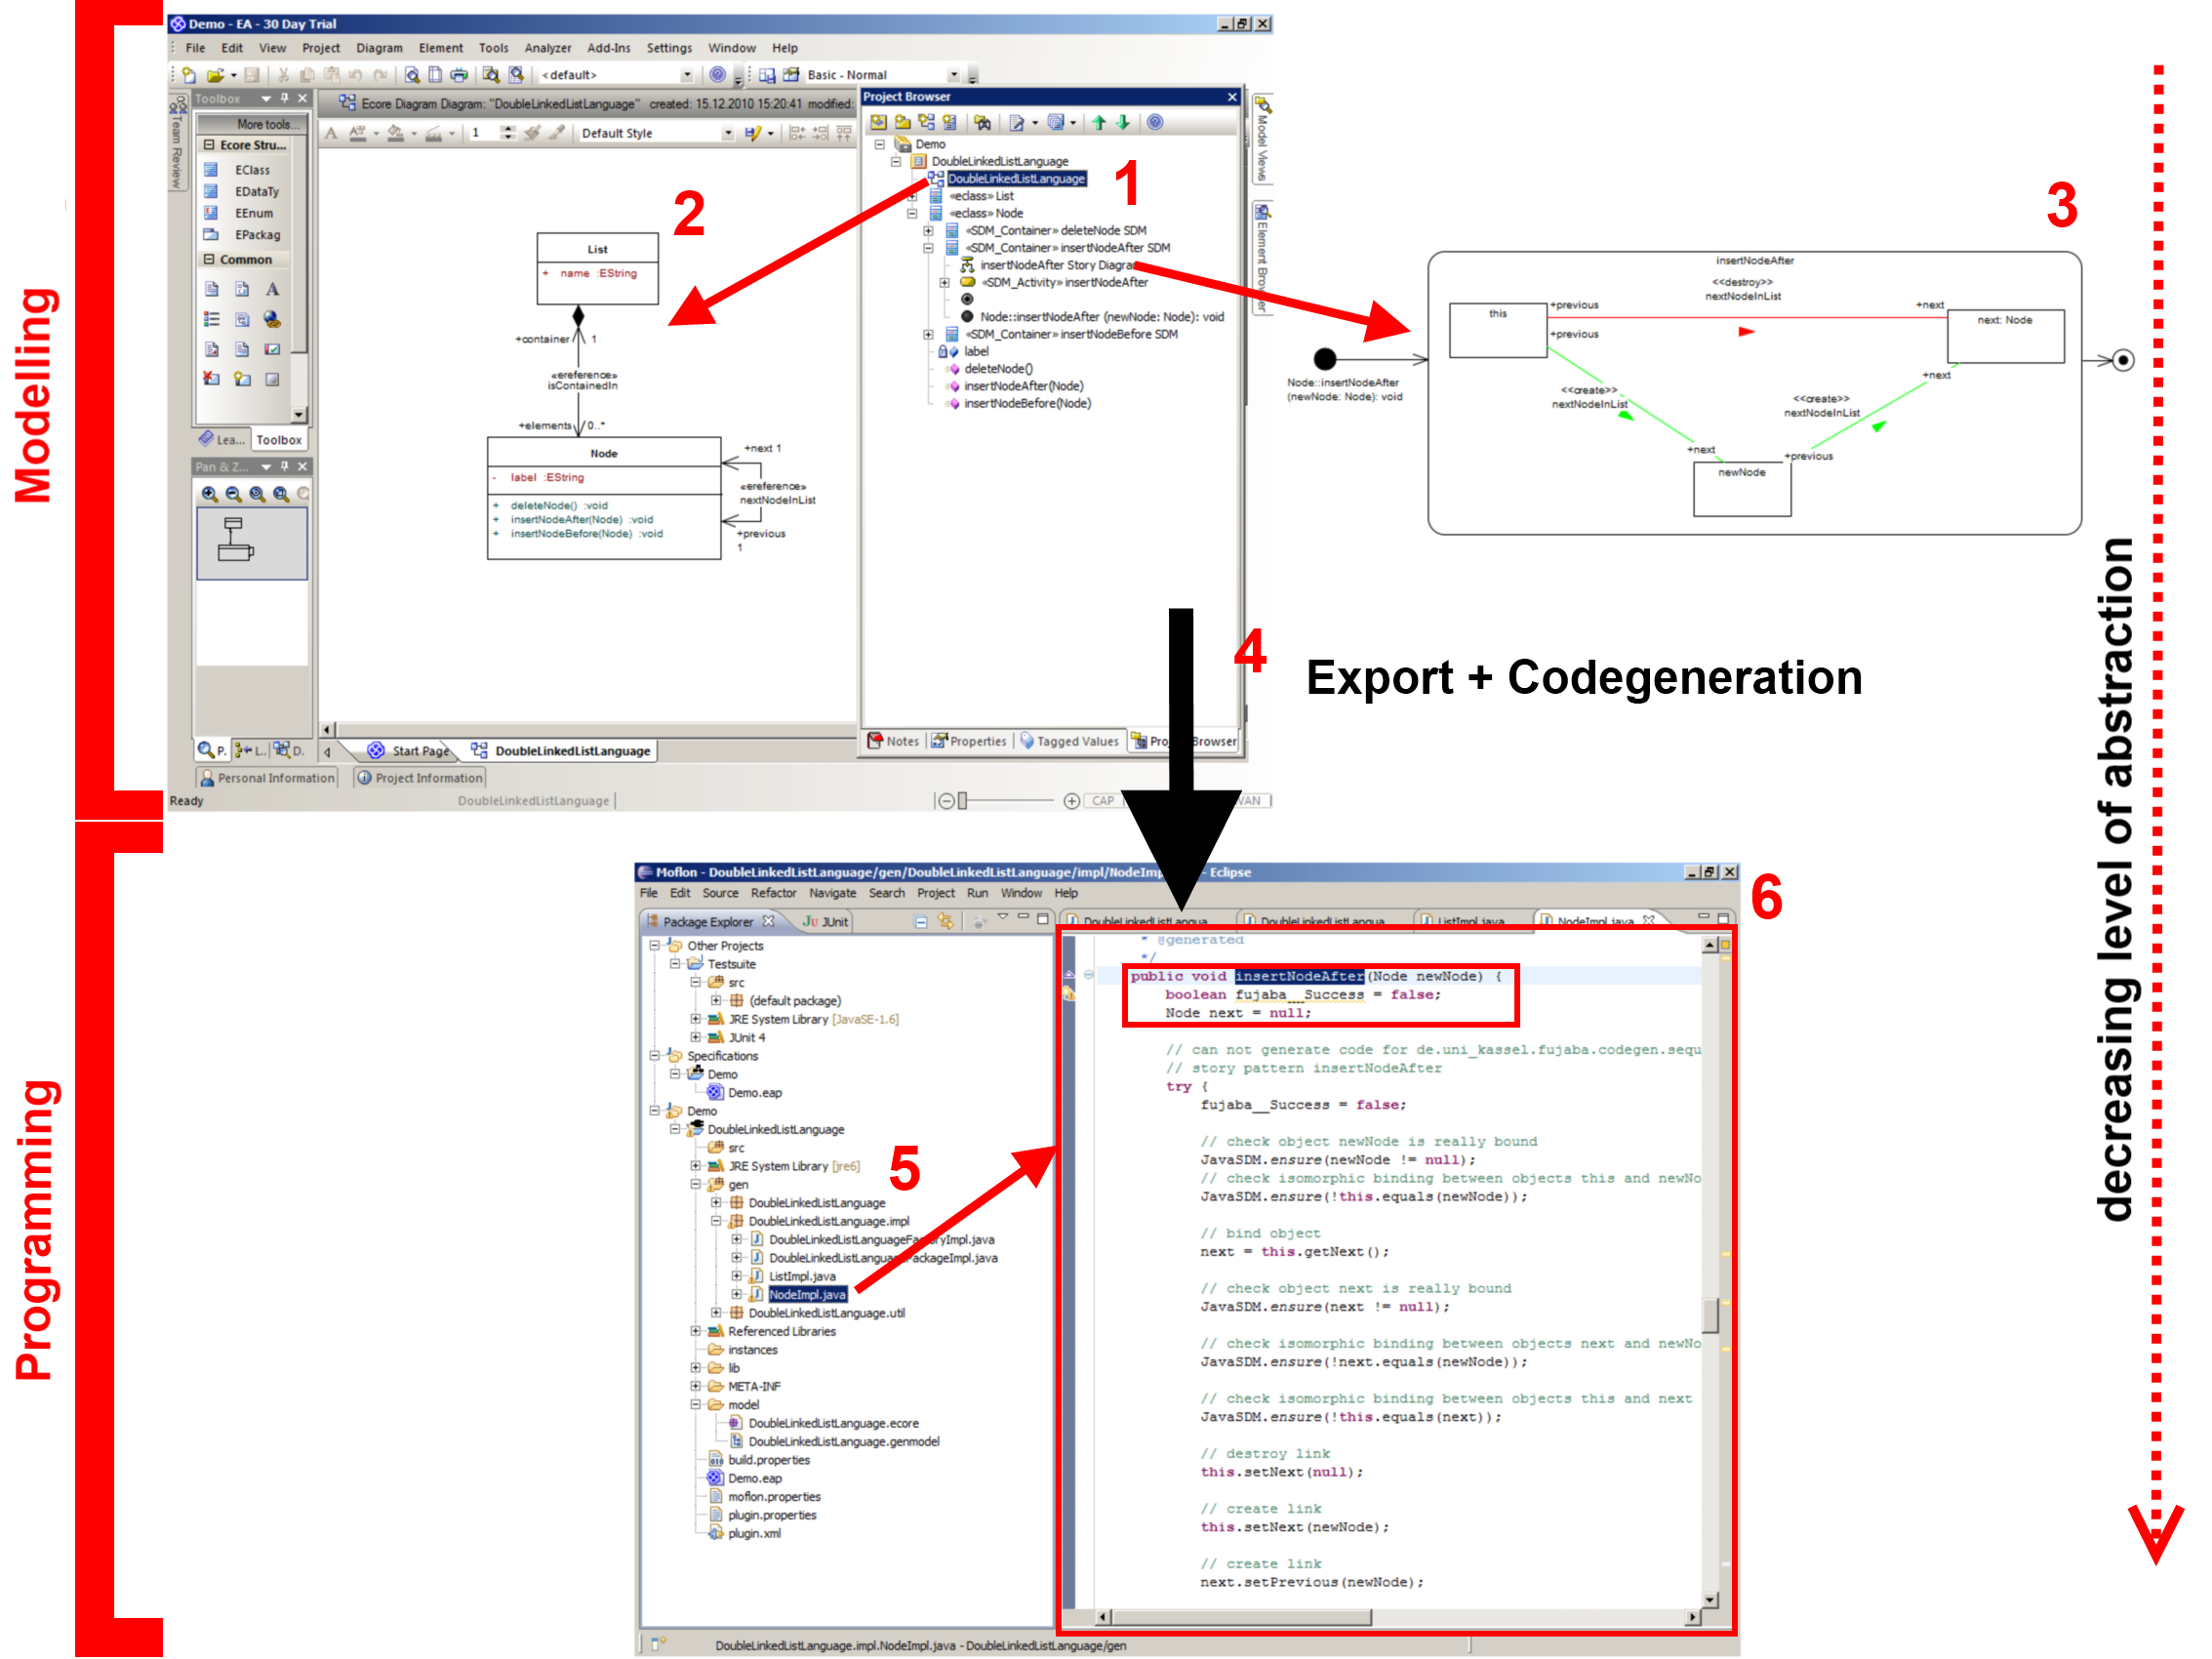
\includegraphics[width=1\textwidth]{pics/installationAndSetup/tafelbild}
	\caption{Overview}
	\label{fig_Overview}
\end{figure}